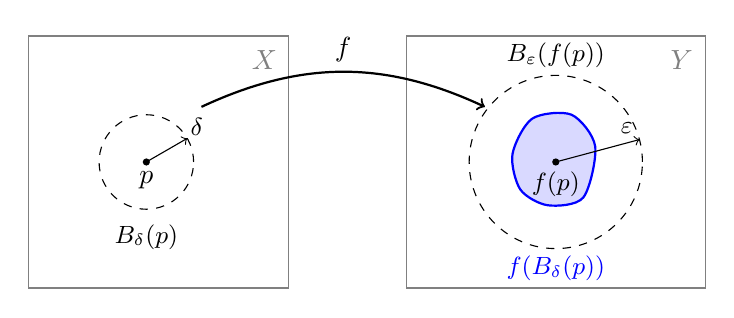
\begin{tikzpicture}
  % domain X
  \draw[gray] (-0.3,-1.6) rectangle (3.0,1.6);
  \node[gray] at (2.7,1.3) {$X$};
  \coordinate (p) at (1.2,0);
  \draw[dashed] (p) circle (0.6);
  \fill (p) circle (1.3pt) node[below] {$p$};
  \draw[->] (p) -- ++(30:0.6) node[above right, inner sep=1pt] {\small $\delta$};
  \node at (1.2,-0.95) {\small $B_\delta(p)$};
  % codomain Y
  \draw[gray] (4.5,-1.6) rectangle (8.3,1.6);
  \node[gray] at (8.0,1.3) {$Y$};
  \coordinate (fp) at (6.4,0);
  \draw[dashed] (fp) circle (1.1);
  \draw[blue, thick, fill=blue, fill opacity=0.15] plot[smooth cycle] coordinates {(5.85,0.1) (6.1,0.55) (6.6,0.6) (6.9,0.2) (6.75,-0.45) (6.3,-0.55) (5.95,-0.35)};
  \fill (fp) circle (1.3pt) node[below] {\small $f(p)$};
  \draw[->] (fp) -- ++(15:1.1) node[pos=0.85, above] {\small $\varepsilon$};
  \node[blue] at (6.4,-1.35) {\small $f(B_\delta(p))$};
  \node at (6.4,1.35) {\small $B_\varepsilon(f(p))$};
  \draw[->, thick] (1.9,0.7) to[bend left=25] node[above] {$f$} (5.5,0.7);
\end{tikzpicture}
